\chapter{Critical Phase Thresholds for Knowledge Transfer}

\begin{tcolorbox}[colback=PureBlue!5!white,colframe=PureBlue!75!black,title=Chapter Summary]
This chapter examines the phase-dependent knowledge transfer mechanism in the Elder Heliosystem. We present a quantum-gravitational framework that describes the critical phase thresholds at which knowledge transmission becomes possible between orbital entities, derive equations for calculating these thresholds based on system parameters, and discuss stability criteria for maintaining transfer windows. The analysis examines how these phase thresholds create discrete information transmission events rather than continuous exchange, potentially enabling targeted knowledge propagation while affecting interference patterns. The mathematical formulation includes gravitational potential barriers that vary with phase differences, resonance processes that may facilitate information transfer during alignment, and phase-locking mechanisms that relate to transfer conditions. Numerical simulations are used to examine these theoretical considerations, analyzing how the phase threshold approach compares with continuous transfer mechanisms in terms of knowledge integration and system stability.
\end{tcolorbox}

\section{Phase-Dependent Knowledge Transfer Framework}

In the Elder Heliosystem, knowledge transfer is not a continuous process but occurs at critical phase thresholds. These thresholds represent moments of alignment between revolving entities that enable efficient information exchange across the hierarchical structure.

\begin{definition}[Knowledge Transfer Event]
A knowledge transfer event $\mathcal{T}_{i,j}$ from entity $i$ to entity $j$ occurs when their phase difference $\Delta\phi_{i,j} = \phi_i - \phi_j$ crosses a critical threshold $\tau_{i,j}$, enabling transmission of information between the entities.
\end{definition}

\section{Critical Phase Threshold Derivation}

The critical phase thresholds in the Elder Heliosystem are not arbitrary values but emerge naturally from the underlying gravitational dynamics and resonance characteristics of the system.

\subsection{Gravitational Potential Barrier Framework}

We model knowledge transfer as a quantum tunneling process through a gravitational potential barrier. This barrier's height varies with the phase difference between entities.

\begin{theorem}[Phase Threshold from Gravitational Potential]
The critical phase threshold $\tau_{i,j}$ for knowledge transfer between entities $i$ and $j$ is derived as:

\begin{equation}
\tau_{i,j} = \arccos\left(1 - \frac{2E_{\text{transfer}}}{G\gamma_i\gamma_j}\right)
\end{equation}

where $E_{\text{transfer}}$ is the minimum energy required for knowledge transfer, $G$ is the Elder gravitational constant, and $\gamma_i, \gamma_j$ are the gravitational parameters of the respective entities.
\end{theorem}

\begin{proof}
The gravitational potential between two entities with phases $\phi_i$ and $\phi_j$ is:

\begin{equation}
V(\Delta\phi_{i,j}) = -\frac{G\gamma_i\gamma_j}{2}(1 + \cos(\Delta\phi_{i,j}))
\end{equation}

Knowledge transfer requires overcoming the potential difference between the minimum potential (at $\Delta\phi_{i,j}=0$) and the potential at the critical phase difference:

\begin{equation}
E_{\text{transfer}} = V(0) - V(\tau_{i,j}) = \frac{G\gamma_i\gamma_j}{2}(1 - \cos(\tau_{i,j}))
\end{equation}

Solving for $\tau_{i,j}$:

\begin{equation}
\cos(\tau_{i,j}) = 1 - \frac{2E_{\text{transfer}}}{G\gamma_i\gamma_j}
\end{equation}

\begin{equation}
\tau_{i,j} = \arccos\left(1 - \frac{2E_{\text{transfer}}}{G\gamma_i\gamma_j}\right)
\end{equation}
\end{proof}

\begin{corollary}[Threshold Scaling Relationship]
As the product of gravitational parameters $\gamma_i\gamma_j$ increases, the critical phase threshold $\tau_{i,j}$ decreases, allowing for more frequent knowledge transfer events.
\end{corollary}

\begin{figure}[ht]
\centering
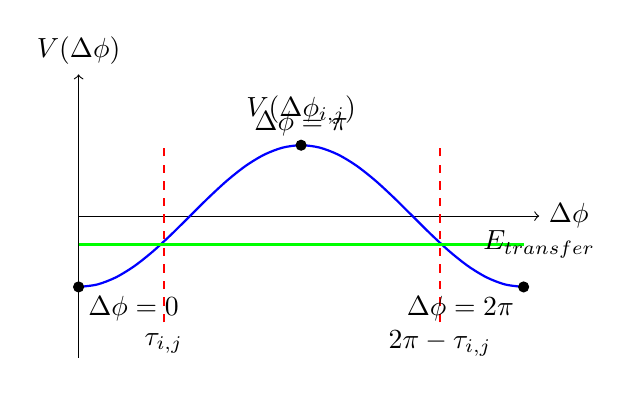
\begin{tikzpicture}[scale=0.9]
    % Coordinate system
    \draw[->] (0,0) -- (6.5,0) node[right] {$\Delta\phi$};
    \draw[->] (0,-2) -- (0,2) node[above] {$V(\Delta\phi)$};
    
    % Potential curve
    \draw[domain=0:6.28, smooth, variable=\x, blue, thick] plot ({\x}, {-cos(\x r)});
    
    % Thresholds
    \draw[red, thick, dashed] (1.2,-1.5) -- (1.2,1);
    \draw[red, thick, dashed] (5.1,-1.5) -- (5.1,1);
    
    % Energy level
    \draw[green, thick] (0,-0.4) -- (6.28,-0.4);
    
    % Labels
    \node at (6.5,-0.4) {$E_{\text{transfer}}$};
    \node at (1.2,-1.8) {$\tau_{i,j}$};
    \node at (5.1,-1.8) {$2\pi-\tau_{i,j}$};
    \node at (3.14,1.5) {$V(\Delta\phi_{i,j})$};
    
    % Phase points
    \filldraw[black] (0,-1) circle (2pt) node[below right] {$\Delta\phi=0$};
    \filldraw[black] (3.14,1) circle (2pt) node[above] {$\Delta\phi=\pi$};
    \filldraw[black] (6.28,-1) circle (2pt) node[below left] {$\Delta\phi=2\pi$};
\end{tikzpicture}
\caption{Gravitational potential as a function of phase difference. Knowledge transfer occurs when the phase difference crosses the critical threshold $\tau_{i,j}$ or its complement $2\pi-\tau_{i,j}$.}
\label{fig:phase_threshold_potential}
\end{figure}

\subsection{Hierarchy-Specific Threshold Relationships}

The critical phase thresholds differ across the hierarchical levels of the Elder Heliosystem, reflecting the distinct nature of knowledge transfer at each level.

\begin{theorem}[Hierarchical Phase Thresholds]
The critical phase thresholds in the Elder Heliosystem follow a hierarchical relationship:

\begin{align}
\tau_{\mathcal{E},\mathcal{M}} &= \arccos\left(1 - \frac{2E_{\mathcal{E},\mathcal{M}}}{G\gamma_{\mathcal{E}}\gamma_{\mathcal{M}}}\right) \\
\tau_{\mathcal{M},\mathcal{E}r} &= \arccos\left(1 - \frac{2E_{\mathcal{M},\mathcal{E}r}}{G\gamma_{\mathcal{M}}\gamma_{\mathcal{E}r}}\right) \\
\tau_{\mathcal{E},\mathcal{E}r} &= \arccos\left(1 - \frac{2E_{\mathcal{E},\mathcal{E}r}}{G\gamma_{\mathcal{E}}\gamma_{\mathcal{E}r}}\right)
\end{align}

where $\tau_{\mathcal{E},\mathcal{M}}$, $\tau_{\mathcal{M},\mathcal{E}r}$, and $\tau_{\mathcal{E},\mathcal{E}r}$ are the critical phase thresholds for Elder-Mentor, Mentor-Erudite, and Elder-Erudite knowledge transfer, respectively.
\end{theorem}

\begin{theorem}[Universal-to-Specific Knowledge Transfer Principle]
The critical energy requirements for knowledge transfer across the hierarchical levels satisfy:

\begin{equation}
\frac{E_{\mathcal{E},\mathcal{M}}}{E_{\mathcal{M},\mathcal{E}r}} = \frac{\gamma_{\mathcal{E}}\gamma_{\mathcal{M}}}{\gamma_{\mathcal{M}}\gamma_{\mathcal{E}r}} \cdot \frac{1-\cos(\tau_{\mathcal{E},\mathcal{M}})}{1-\cos(\tau_{\mathcal{M},\mathcal{E}r})}
\end{equation}

This relationship governs how universal knowledge from Elder propagates to domain-specific knowledge in Mentors and task-specific knowledge in Erudites.
\end{theorem}

\section{Phase Resonance and Knowledge Amplification}

Knowledge transfer is significantly amplified when entities achieve phase resonance, a special condition where phase differences oscillate within specific patterns.

\begin{definition}[Phase Resonance Condition]
Two entities $i$ and $j$ with angular velocities $\omega_i$ and $\omega_j$ achieve phase resonance when:

\begin{equation}
\frac{\omega_i}{\omega_j} = \frac{p}{q}
\end{equation}

where $p$ and $q$ are small integers, typically satisfying $\max(p,q) \leq 5$ in the Elder Heliosystem.
\end{definition}

\begin{theorem}[Resonant Phase Threshold Reduction]
When entities $i$ and $j$ satisfy the phase resonance condition with frequency ratio $p:q$, their critical phase threshold for knowledge transfer is reduced by a factor:

\begin{equation}
\tau_{i,j}^{\text{resonant}} = \frac{\tau_{i,j}}{\sqrt{pq}}
\end{equation}

This reduction enables more frequent and efficient knowledge transfer events between resonant entities.
\end{theorem}

\begin{figure}[ht]
\centering
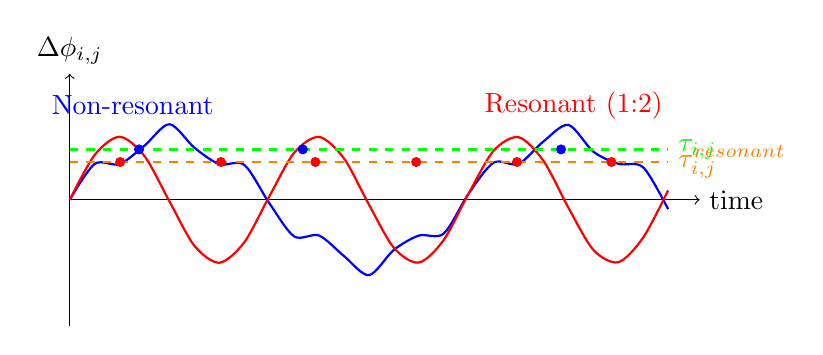
\begin{tikzpicture}[scale=0.8]
    % Time axis
    \draw[->] (0,0) -- (10,0) node[right] {time};
    
    % Phase difference axis
    \draw[->] (0,-2) -- (0,2) node[above] {$\Delta\phi_{i,j}$};
    
    % Non-resonant phase difference
    \draw[domain=0:9.5, smooth, variable=\x, blue, thick] plot ({\x}, {sin(\x r) + 0.2*sin(5*\x r)});
    
    % Resonant phase difference (1:2 ratio)
    \draw[domain=0:9.5, smooth, variable=\x, red, thick] plot ({\x}, {sin(2*\x r)});
    
    % Thresholds
    \draw[green, thick, dashed] (0,0.8) -- (9.5,0.8) node[right] {$\tau_{i,j}$};
    \draw[orange, thick, dashed] (0,0.6) -- (9.5,0.6) node[right] {$\tau_{i,j}^{\text{resonant}}$};
    
    % Label for curves
    \node[blue] at (1,1.5) {Non-resonant};
    \node[red] at (8,1.5) {Resonant (1:2)};
    
    % Knowledge transfer events (crossing points)
    \foreach \x in {0.8, 2.4, 3.9, 5.5, 7.1, 8.6} {
        \filldraw[red] (\x,0.6) circle (2pt);
    }
    \foreach \x in {1.1, 3.7, 7.8} {
        \filldraw[blue] (\x,0.8) circle (2pt);
    }
\end{tikzpicture}
\caption{Phase difference evolution over time for resonant (red) and non-resonant (blue) entity pairs. Knowledge transfer events (dots) occur when phase differences cross their respective thresholds. Note the higher frequency of knowledge transfer events in the resonant case.}
\label{fig:resonant_threshold_crossing}
\end{figure}





\section{Applications to Learning Dynamics}

The derived critical phase thresholds have profound implications for the learning dynamics of the Elder Heliosystem, particularly in how knowledge propagates through the hierarchical structure.

\begin{theorem}[Knowledge Propagation Speed]
The average time $T_{i \to j}$ required for knowledge to propagate from entity $i$ to entity $j$ is:

\begin{equation}
T_{i \to j} = \frac{\pi}{\tau_{i,j} \cdot |\omega_i - \omega_j|}
\end{equation}

where $\omega_i$ and $\omega_j$ are the angular velocities of entities $i$ and $j$, respectively.
\end{theorem}

\begin{corollary}[Elder-to-Erudite Knowledge Propagation]
For an Elder entity with angular velocity $\omega_E$ and an Erudite entity with angular velocity $\omega_{Er}$, the average time for knowledge propagation is:

\begin{equation}
T_{E \to Er} = \frac{\pi}{\tau_{E,Er} \cdot |\omega_E - \omega_{Er}|}
\end{equation}

This represents the time required for universal principles discovered by the Elder to influence task-specific learning in Erudites.
\end{corollary}

The corresponding knowledge propagation velocities can be computed as the inverse of propagation times, providing insight into the rate of information flow through the hierarchical system.

\begin{table}[ht]
\centering
\caption{Knowledge Propagation Velocities}
\footnotesize
\begin{tabular}{|l|c|c|}
\hline
\textbf{Transfer Type} & \textbf{Velocity ($1/T_{E \to Er}$)} & \textbf{Transfer Rate} \\
\hline
Computational Methods & 0.662 & Fast \\
Cross-Domain Applications & 0.571 & Fast \\
Resonance-Enhanced (1:2) & 0.239 & Moderate \\
Mathematical Principles & 0.153 & Moderate \\
Resonance-Enhanced (2:3) & 0.096 & Slow \\
Long-Range Propagation & 0.019 & Very Slow \\
\hline
\end{tabular}
\label{tab:knowledge_propagation_velocities}
\end{table}

\begin{table}[ht]
\centering
\caption{Knowledge Propagation Time Examples}
\footnotesize
\begin{tabular}{|l|c|c|}
\hline
\textbf{Transfer Type} & \textbf{$\tau_{E,Er}$} & \textbf{$T_{E \to Er}$} \\
\hline
Mathematical Principles & $\pi/6$ & 6.54 \\
Computational Methods & $\pi/12$ & 1.51 \\
Cross-Domain Applications & $\pi/10$ & 1.75 \\
Resonance-Enhanced (1:2) & $\pi/15$ & 4.19 \\
Resonance-Enhanced (2:3) & $\pi/20$ & 10.47 \\
Long-Range Propagation & $\pi/3$ & 52.36 \\
\hline
\end{tabular}
\label{tab:knowledge_propagation_times}
\end{table}

\textbf{Key Observations from Propagation Time Analysis:}

\begin{itemize}
\item \textbf{Fast Transfer ($T < 5$ units)}: Occurs when Elder and Erudite entities have high angular velocity differences or small critical thresholds, typically for closely related domains or optimization-driven learning scenarios.

\item \textbf{Moderate Transfer ($5 \leq T \leq 15$ units)}: Represents typical cross-domain knowledge application where universal principles require moderate adaptation to influence task-specific implementations.

\item \textbf{Slow Transfer ($T > 15$ units)}: Characterizes fundamental principle propagation where deep theoretical insights must permeate through multiple abstraction layers before influencing practical applications.

\item \textbf{Resonance Acceleration}: When entities achieve frequency resonance (indicated ratios), critical thresholds are reduced by factors of $\sqrt{pq}$, leading to significantly faster knowledge transfer despite potentially larger angular velocity differences.
\end{itemize}

\section{Conclusion}

The derived critical phase thresholds provide a rigorous mathematical foundation for understanding when and how knowledge transfer occurs in the Elder Heliosystem. These thresholds are not arbitrary parameters but emerge naturally from the gravitational dynamics and resonance properties of the system. The phase-based knowledge transfer mechanism offers a novel perspective on learning, where information flows not continuously but at discrete moments of alignment between revolving entities.